% document type
\documentclass[12pt]{article}

% packages
\usepackage[total={170mm,230mm}]{geometry}
\usepackage[utf8]{inputenc}
\usepackage[T2A]{fontenc}
\usepackage[russian]{babel}
\usepackage{graphicx}
\usepackage{xcolor}
\usepackage{amssymb}
\usepackage{amsfonts}
\usepackage{amsmath}
\usepackage{amsthm}
\usepackage{physics}
\usepackage{nicefrac}
\usepackage{wrapfig}
\usepackage{cancel}
\usepackage{hyperref, cmap}
\usepackage{pgfplots}

% settings
\pgfplotsset{width=\linewidth, compat=newest}

% definitions
\DeclareMathOperator\arctanh{arctanh}
\DeclareMathOperator\arccosh{arccosh}
\DeclareMathOperator\const{const}
\newtheorem{definition}{Опредление}[section]
\newtheorem{theorem}{Теорема}[section]
\newtheorem{axiom}{Аксиома}[section]
\newtheorem{hypothesis}{Гипотеза}[section]

\title{Исследование полиномов}
\author{Алексей Савватеев \and Александр Тонис}

\begin{document}
\maketitle
\begin{abstract}
В данной лекции детально изучены многочлены, сформулирована и доказана теорема Безу, исследованы первая и более старшие производные многосленов, продемонстрированы различные способы нахождения точек локального максимума и минима, кроме того, подробно рассмотрены примеры исследования функций и построяния их графиков.
\par
Конспектировал Александр Козлов. 
\end{abstract}
\newpage
\tableofcontents
\newpage
\section{Многочлены и их графики}
Математический анализ отличается от математики, изучаемой в школе, во\--первых, тем, что математический анализ оперирует понятием предела (см. \cite{lim_use}), во\--вторых, тем, что в математическом анализе рассматривают объекты различной размерности, а не только одномерные. Проиллюстрируем эти различия на примере многочленов. Напомним читателю некоторые важные факты о многочленах. Прежде всего введём определение многочлена.

\begin{definition}
	Многочленом натуральной степени $n$ называется функция, представляющая из себя сумму следующего вида:
	\begin{equation}
	f(x) = \sum_{k=0}^n{a_k \cdot x^k},
	\end{equation}
	где $a_n$ не равно нулю.
\end{definition}

Важно заметить, что если $a_k$ было равно нулю, то многочлен не зависит от $k$\--ой степени аргумента $x$. Поэтому в определении многочлена степени $n$ присутствует требование

\begin{equation}
a_n \ne 0.
\end{equation}

\par
Качественно изучим график многочлена некоторой натуральной степени. Можно заметить, что если старший коэффициент ($a_n$) положительный, то при стремлении аргумента $x$ к плюс бесконечности многочлен степени $n$ неограниченно растёт (см. рис. \ref{fig:1}), что можно записать следующим образом:

\begin{equation}
f(x) = \sum_{k=0}^n{a_k \cdot x^k} \underset{x\rightarrow+\infty}{\longrightarrow}+\infty.
\end{equation}

\begin{figure}[htbp]
  \label{fig:1}
	\centering
	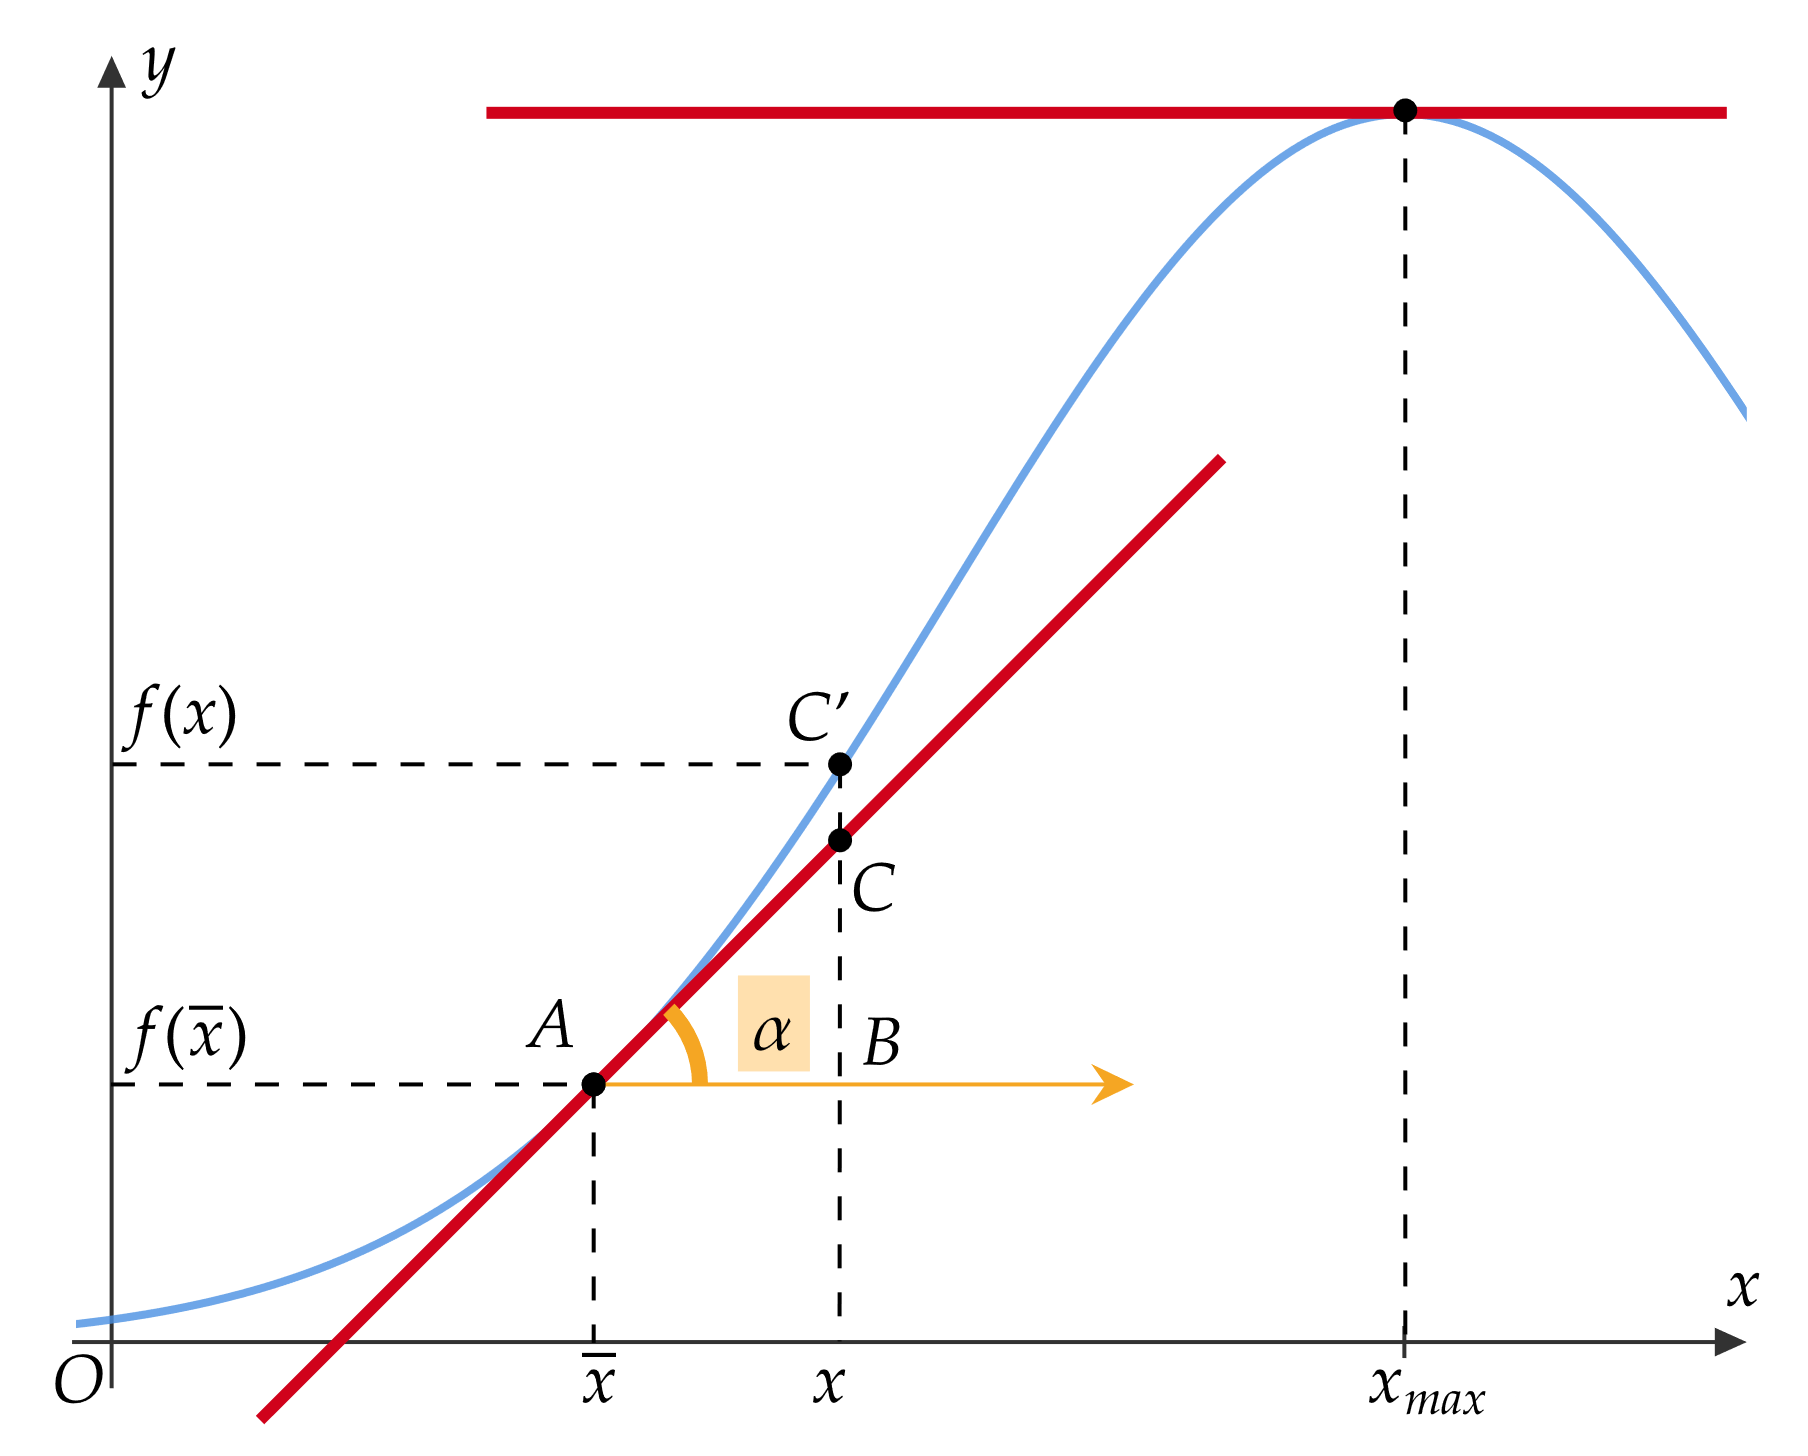
\includegraphics[width=1\linewidth]{fig1}
	\caption{График полиномов нечетной степени. В синий цвет окрашен график функции $2x^{7} - 28 x^{5} + 98 x^{3} - 72 x$, в зелёный~\----~график функции $x^{7} - 14 x^{5} + 49 x^{3} - 36 x$. Пунктирная синяя кривая является графиком функции $-2x^{7} + 28 x^{5} -98 x^{3} + 72 x$. Видно, что с ростом $x$ синий график неограниченно растёт, синий пунктирный же неограниченно убывает, красный график тоже растёт, как и синий, но медленнее.}
\end{figure}

Действительно, так как все коэффициенты $\qty{a_k}_{k=0}^n$ являются фиксированными величинами, то при росте аргумента быстрее всего растёт слагаемое с наибольшей степенью. Например, рассмотрим функцию

\begin{equation}
f(x)=2x^{7} - 28 x^{5} + 98 x^{3} - 72.
\end{equation}

Уже при $x = 1000$ имеем следующее значение функции:

\begin{equation}
f(1000) = 2 \cdot 10^{21} - 28 \cdot 10^{15} + 98 \cdot 10^9 - 72.
\end{equation}

Видно, что \emph{старшее} слагаемое (слагаемое большей степени) на несколько порядков (в несколько миллионов раз) превосходит остальные слагаемые по абсолютному значению, то есть все слагаемые, кроме главного члена, вносят незначительный вклад в значение функции. Главный член многочлена с ростом $x$ продолжает увеличиваться, затмевает собой остальные члены, поэтому функция неограниченно растёт.

\par
Представляется очевидным такой вывод. Если коэффициент при главном члене многочлена будет отрицательным, то и стремиться выражение будет к отрицательной бесконечности (см. рис. \ref{fig:1}).

\par 
Мы установили, что знак бесконечности, к которой стремится значение многочлена $f(x)$ при стремлении $x$ к положительной бесконечности, определяется только знаком старшего коэффициента. При рассмотрении 

\begin{equation}
x\rightarrow-\infty
\end{equation}

предел, к которому стремится $f(x)$ начинает зависеть ещё и от степени многочлена. Так, например, из рисунка \ref{fig:1} видно, что при положительном старшем коэффициенте и нечетной степени многочлена 

\begin{equation}
	f(x) \underset{x\rightarrow-\infty}{\longrightarrow}-\infty.
\end{equation}

Ясно, что при отрицательном $a_n$ стремиться многочлен при неограниченном уменьшении $x$ будет к плюс бесконечности. То есть \emph{при нечетной степени многочлена его "хвосты" (ветки, уходящие на бесконечности) направлены в разные стороны}. 

\par 
А что будет при четной степени многочлена? Установим ответ на данный вопрос, обратившись к простому примеру. Если вспомнить график параболы $x^2$ (см. рис. \ref{fig:2}), то можно заметить, что \emph{"хвосты" графика направлены в одном направлении}. Это общий результат для всех многочленов четного порядка и связан он с тем, что $\qty(x)^2 = \qty(-x)^2$, то есть для четных степеней знак аргумента в рассматриваемом вопросе не важен. 

\begin{figure}[htbp]
\centering
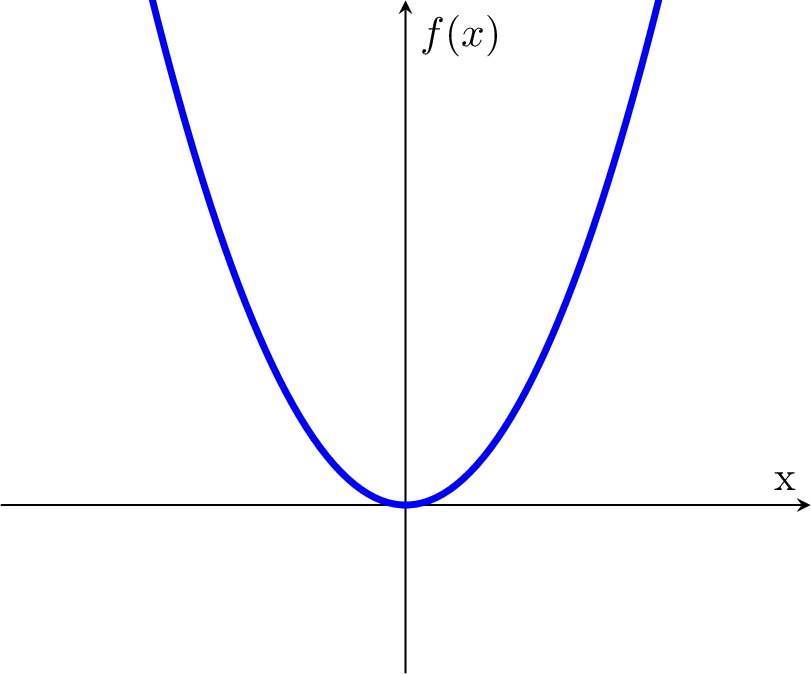
\includegraphics[width=1\linewidth]{fig2}
\caption{График параболы.}
\label{fig:2}
\end{figure}

\par
Одной из основных задач алгебры является задача поиска корней уравнения типа

\begin{equation}\label{eq:1}
\sum_{k=0}^n{a_k \cdot x^k} = 0.
\end{equation}

То есть рассматривается уравнение, представляющее из себя многочлен степени $n$, приравненный к нулю. В силу свойств уравнений, можно поделить равенство (\ref{eq:1}) на значение старшего коэффициента $a_n$, благо оно отлично от нуля в силу определения многочлена степени $n$. Тогда получим \emph{приведённый} многочлен, который можно записать так:

\begin{equation}\label{eq:2}
\sum_{k=0}^{n-1}{\dfrac{a_k}{a_n} \cdot x^k} + x^n = 0.
\end{equation}

Уравнения (\ref{eq:1}) и (\ref{eq:2}) тождественны друг другу, что означает совпадение их корней. А как при этом соотносятся графики многочленов? Вновь обратимся к рисунку \ref{fig:1}. На нём видно, что при пропорциональном уменьшении всех коэффициентов многочлена на одно и тоже число (то есть при делении многочлена на число, большее единицы) график многочлена прижимается к оси абсцисс, поведение функции при этом не меняется, то есть точки экстремума не меняют своего положения и сохраняется направление роста при стремлении $x$ к бесконечностям.

\section{Теорема Безу}
Посмотрим для начала на рисунок \ref{fig:1}, графики всех функций пересекают ось абсцисс ровно семь раз. Это означает, что функции имеют семь корней. Оказывается, если полином имеет семь корней, то можно утверждать, что степень данного полинома больше либо равна семи. Как будет показано дальше такой вывод следует из теоремы Безу. То есть просто по количеству корней возможно получить ограничение на степень полинома.

\subsection{Формулировка и доказательство}
Чтобы логично подступить к формулировке рассматриваемой теоремы, поговорим сперва о делении многочленов с остатком (бегло вспомнить данную тему повожет Wikipedia \cite{poly_div}). Если многочлен степени $n$ делится на линейную функцию $x-a$ с остатком $b$, то это равносильно такой записи:

\begin{equation}
\sum_{k=0}^n{a_k \cdot x^k} = \sum_{k=0}^{n-1}{b_k x^k}\cdot \qty(x-a) + b.
\label{eq:3}
\end{equation}

Из данного соотношения и следует теорема Безу, формулирующаяся следующим образом.

\begin{theorem}
	Число $a$ является корнем многочлена $f(x)$ тогда и только тогда, когда $f(x)$ делится без остатка на $(x-a)$.
\end{theorem}

\begin{proof}
Пускай $f(x)$ делится без остатка на $(x-a)$, тогда 

\begin{equation}
f(x) = \sum_{k=0}^n{a_k \cdot x^k} = \sum_{k=0}^{n-1}{b_k x^k}\cdot \qty(x-a).
\end{equation}

Очевидно, что если подставить в правую часть $x=a$, то получим $0$, что и требовалось доказать. 

\par 
Мы доказали теорему только с одной стороны, так как мы утверждаем эквивалентность двух утверждений, то требуется доказательство и с другого подступа. Пускай теперь число $a$ является корнем многочлена $f(x)$. Тогда остаётся верным равенство (\ref{eq:3}), откуда при $x=a$ получаем

\begin{equation}
  f(a) = \sum_{k=0}^n{a_k \cdot a^k} = \sum_{k=0}^{n-1}{b_k a^k}\cdot \qty(a-a) + b = b.
\end{equation}

Но левая часть равна нулю, значит и $B = 0$. Значит, делится многочлен на $(x-a)$ без остатка.
\end{proof}

\subsection{Следствие}
Из приведённой теоремы сущетсвует следствие, о котором говорилось в начале лекции. Прийдём к нему методом математической индукции. Сначала рассмотрим некоторый полином $f_{(1)}(x)$ неизвестной нам степени $n$, имеющий один корень $x=c_1$. Для такого полинома работает теорема Безу, из которой следует

\begin{equation}
  f_{(1)}(x) = g_1(x)\cdot \qty(x-c_1),
\end{equation}

где $g_1(x)$ является полиномом степени $(n-1)$. Это значит, что степень полинома $f_{(1)}(x)$ должна быть как минимум $1$. 

\par 
Пускай теперь полином $f_{(2)}(x)$ некоторой неизвестной нам степени $n$ имеет два различных действительных корня $c_1$ и $c_2$, тогда сначала применяем теорему Безу для первого корня и получаем равенство

\begin{equation}
  f_{(2)}(x) = g_1(x)\cdot \qty(x-c_1).
\end{equation}

Так как $c_2$ так же является корнем полинома $f_{(2)}(x)$, то 

\begin{equation}
\label{eq:4}
  f_{(2)}(c_2) = g_1(c_2)\cdot \qty(c_2-c_1) = 0.
\end{equation}

Если $c_1 \ne c_2$, то для того, чтобы удовлетварить соотношению (\ref{eq:4}), нужно положить, что $c_2$ является корнем полинома $g_1(x)$. Применяем для $g_1(x)$ те же рассуждения, что были провидены выше для $f_{(1)}(x)$, и получаем

\begin{equation}
  f_{(2)}(x) = g_2(x)\cdot \qty(x-c_2)\cdot \qty(x-c_1).
\end{equation}

Данное равенство означает, что степень полинома $f_{(2)}(x)$ должна быть как миним двойкой.

\par
Если взять два приведённых пример в качестве базиса метода математической индукции, то удастся доказать следующее утверждение.

\begin{theorem}
  Eсли некоторый полином $f_{(m)}(x)$ неизвестной нам степени $n$ имеет $m$ различных корней $\qty{c_k}_{k=1}^m$, то степень полинома $n$ больше либо равна $m$.
\end{theorem}

\section{Производные и локальные экстремумы}
Рассмотрим некоторый приведённый многочлен степени $n$

\begin{equation}
  f(x) = x^n + a_{n-1} x^{n-1} + \ldots + a_1 x + a_0.
\end{equation}

Мы рассматриваем именно приведённый многочлен, так как для настоящих изысканий старший коэффициент не представляет важности (при делении многочлена на старший коэффициент график многочлена может лишь сжаться, либо расстянуться или же зеркально отобразиться около оси абсцисс). Для многих практических задач является важным найти точки максимума либо минимума рассматриваемого полинома. Как редуцировать задачу поиска точек экстремума к задаче о поиске корней многочлена и можно ли это сделать вообще?

\subsection{Производная степенной функции}
\par Чтобы ответить на данный вопрос, нужно ввести понятие производной для степенной функции (ещё раз, прошлые попытки были сделаны на прошлых лекциях \cite{lim_use}). Производная есть мера наклона кривой в данной точке. В качестве меры наклона выбирают тангенс угла наклона. Углом наклона называют угол между положительным направлением оси абсцисс и касательной к графику, проведённой к рассматриваемой точке.

\par Строгое определение производной записывается с помощью предела. 

\begin{definition}\label{def:1}
	Производная функции $f(x)$ обозначается через $f'(x)$ и определеяется следующим образом:
	
	\begin{equation}
		f'(\overline{x}) = \lim_{x\rightarrow\overline{x}}\dfrac{f(x) - f(\overline{x})}{x - \overline{x}}.
	\end{equation}
\end{definition}

\par То есть это ни что иное, как тангенс угла наклона. Действительно, из рисунка \ref{fig:fig1} видно, что если стремить точку $x$ к $\overline{x}$, то точка $C'$ будет стремиться к $C$, то есть тангенс угла $\measuredangle BAC'$ будет стремиться к тангенсу угла наклона $\measuredangle BAC$.

\begin{figure}[htbp]
	\centering
	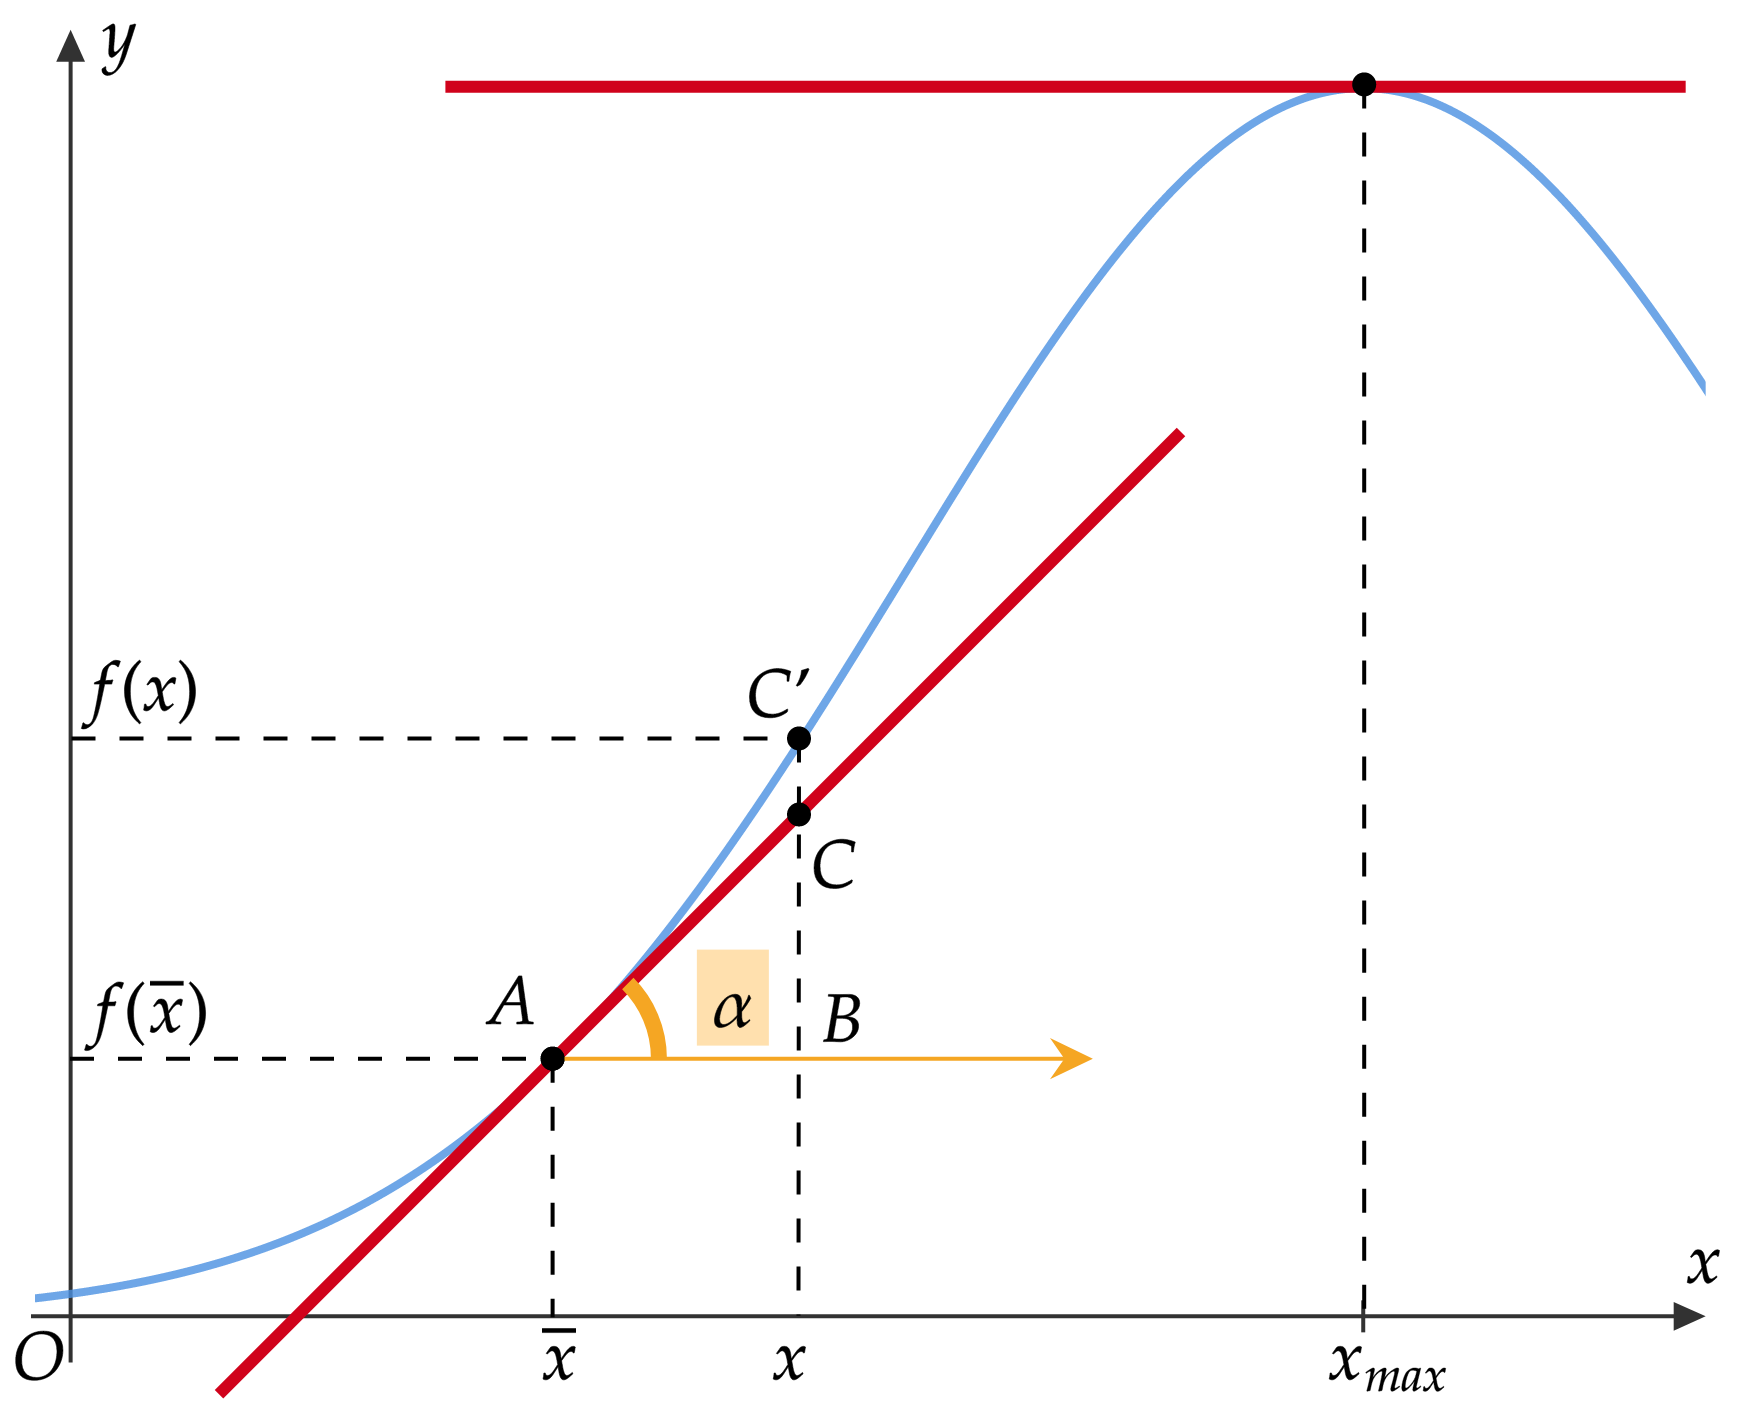
\includegraphics[width=1\linewidth]{fig3}
	\caption{График некоторого полинома. Красным обозначены касательные в графику. Желтой стрелкой обозначаётся положительное направление оси абсцисс.}
	\label{fig:fig1}
\end{figure}

\par Посчитаем по определению \ref{def:1} производную функции $f(x) = x^n$, где под $n$ понимается натуральное число. Общая идея вычисления производных по определению заключается в том, что нужно избыть неопределённость типа $0/0$ под знаком придела. Такая неопределённость появляется прямо из определения \ref{def:1}, ведь, очевидно, что пределы числителей и знаменателей равны нулю. Чтобы избыть данную неопределённость нужно сократить на общий множитель (который и стремиться к нулю) числитель и знаменатель.

\par Проиллюстрируем этот принцип с помощью вычисления производной от степенной функции $f(x) = x^n$. Для этого воспользуемся формулой сокращенного умножения \cite{sok_um} для разности $n$\--ых степеней

\begin{equation}
	a^n - b^n = (a-b)\cdot(a^{n-1} + a^{n-2}b + \ldots + ab^{n-2} + b^{n-1}).
\end{equation}

Тогда можно вычислить производную следующим образом:

\begin{equation}\label{eq:69}
\begin{split}
	f'(\overline{x}) &= \lim_{x\rightarrow\overline{x}}\dfrac{x^n - \overline{x}^n}{x - \overline{x}}\\
	&= \lim_{x\rightarrow\overline{x}} \dfrac{(x-\overline{x}^n)\cdot(x^{n-1} + x^{n-2}\overline{x} + \ldots + x\overline{x}^{n-2} + \overline{x}^{n-1})}{x - \overline{x}}\\
	&= \lim_{x\rightarrow\overline{x}} x^{n-1} + x^{n-2}\overline{x} + \ldots + x\overline{x}^{n-2} + \overline{x}^{n-1}\\
	&= \overline{x}^{n-1} + \overline{x}^{n-2}\ \overline{x} + \ldots + \overline{x}\ \overline{x}^{n-2} + \overline{x}^{n-1}\\
	&= n \overline{x}^{n-1}.
\end{split}
\end{equation}

Таким образом производной от $n$\--ой степенной функции $x^n$ является тоже степенная функция, только степени на единицу меньше $nx^{n-1}$.

\subsection{Локальные экстремумы}
Локальным экстремум в общем случае называют те точки, в которых касательные параллельны оси абсцисс, то есть те точки, где углы наклона равны $0$. А если угол наклона равен нулю, то и его тангенс равен нулю, значит, производная в точках локального экстремума равна $0$. Отсюда получаем уравнение на корни многочлена, который является производной от исходного многочлена. Это и есть редуцирования задачи о поиске локального экстремума к задаче о поиске корней многочлена.

\par
Действительно, если исследовать многочлен

\begin{equation}
	f(x) = x^n + a_{n-1}x^{n-1} + \ldots + a_2 x^2 + a_1 x + a_0,
\end{equation}

на точки экстремума, то для того, чтобы найти эти точки, нужно найти корни уравнения

\begin{equation}
	f'(x) = n x^{n-1} + (n-1)a_{n-1}x^{n-1} + \ldots + 2 a_2 x + a_1,
\end{equation}

что представляет собой уравнение на корни многочлена $f'(x)$.

\section{Старшие производные}
\subsection{Примеры}
Начнём с некоторых примеров. Рассмотрим сперва обычную параболу $f(x) = x^2$. Возьмём первую производную от данной функции. По формуле (\ref{eq:69}) получаем

\begin{equation}
	\qty(x^2)' = 2 x.
\end{equation}

Не будем останавливаться на достигнутом и попробуем посчитать производную от производной, то есть \emph{вторную производную}. Тогда имеем

\begin{equation}
	\qty(x^2)'' = 2.
\end{equation}

Если посчитать третью производную, то получим

\begin{equation}
	\qty(x^2)''' = 0.
\end{equation}

Все вычисленные производные (отличные от тождественного нуля) изображены на графике \ref{fig:69}.

\begin{figure}[htbp]
\centering
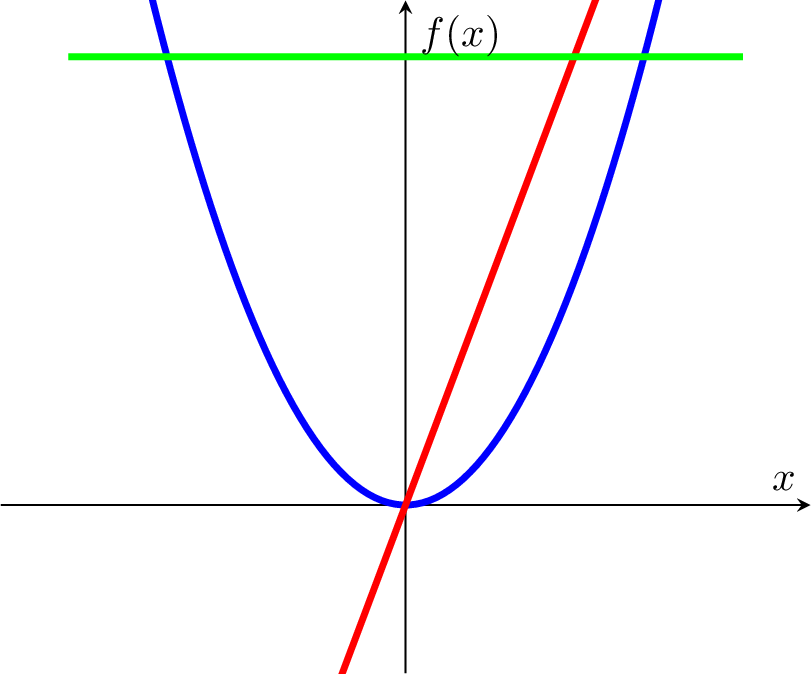
\includegraphics[width=1\linewidth]{fig4}
\caption{График параболы $f(x) = x^2$ изображён синей кривой. Красной кривой обозначен график первой производной $f'(x) = 2x$, а зелённым цветом нарисована вторая производная $f'{}'{}(x)=2$.}
\label{fig:69}
\end{figure}

Рассмотрим теперь параболу в более общем случае, а именно следующую функцию:

\begin{equation}\label{eq:70}
	f(x)=ax^2+bx+c.
\end{equation}

Так как предел суммы равен сумме пределов, то и производная суммы равна сумме производных. Это обстоятельство позволяет нам вычислять производные от суммы степенных функций. Тогда производная от параболы (\ref{eq:70}) будет

\begin{equation}
	f'(x)=2ax+b.
\end{equation}

Вторая же производная запишется следующим образом:

\begin{equation}
	f''(x)=2a.
\end{equation}

Так как вторая производная является константой, то третья будет тождественным нулём, так как угол наклона касательной к функции, которая и так параллельна всюду оси абсцисс, будет нулём, а тангенс от нуля это тоже нуль.

Для конкретного примера 

\begin{equation}
	f(x) = -x^2 + x - 1
\end{equation}

данные производные посчитаны и их графики построены (см. рис. \ref{fig:70}).

\begin{figure}[htbp]
\centering
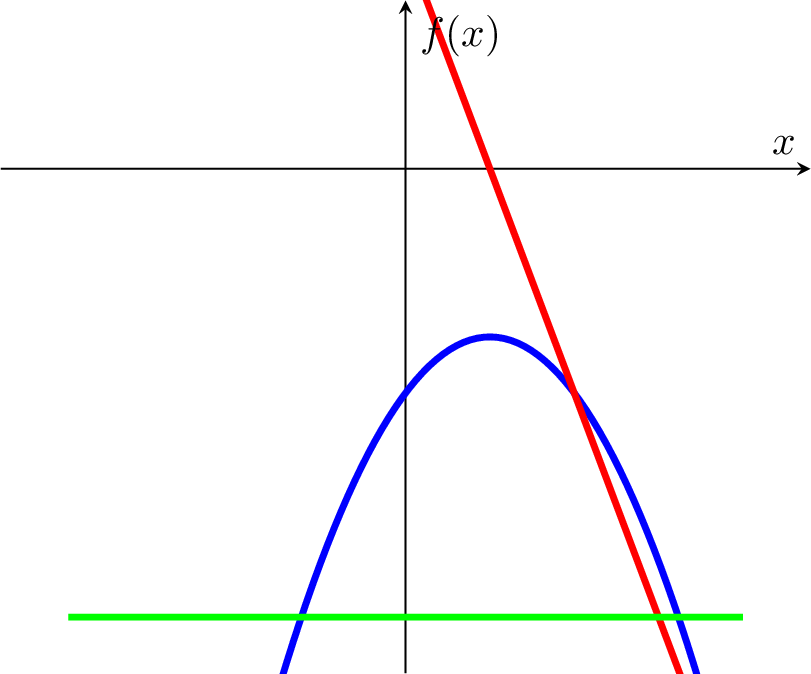
\includegraphics[width=1\linewidth]{fig5}
\caption{График параболы $f(x) = -x^2 + x - 1$ изображён синей кривой. Красной кривой обозначен график первой производной $f'(x) = -2x+1$, а зелённым цветом нарисована вторая производная $f''(x) = -2$.}
\label{fig:70}
\end{figure}

Из приведённых примеров можно вывести (пока что чисто эмпирически, а далее в курсе мы сможем более строго это рассмотреть) следующее утверждение. \emph{Если функция $f(x)$ имеет третью производную равной нулю, то она имеет вид} 

\begin{equation}
	f(x)=ax^2+bx+c.
\end{equation}

\subsection{Смысл производных}
Разберёмся со смыслом производных. Первая производная имеет своим смыслом отражать наклон кривой в данной точке или, что то же самое, скорость роста функции, ведь чем круче идёт кривая, тем быстрее она растёт. Кроме того, отсюда становится ясно, почему в точках локального максимума или минимума, где функция локально никуда не растёт, производная обращается в нуль. 

\par В чём же смысл второй производной? Она является производной от первой производной, следовательно, она отражает скорость роста первой производной, то есть скорость роста скорости роста исходной функции. В кинематике материальной точки на уроках физики в школе такую характеристику именуют ускорением. Там, где скорость роста исходной функции возрастает, вторая производная растёт, где скорость роста начальной функции уменьшается~\----~вторая производная имеет отрицательный знак. Значит, в точках, где скорость роста функции меняет направление роста, вторая производная обращается в нуль.

\par Как знак второй производной влияет на исходную функцию? Обратимся для иллюстрации к рисунку \ref{fig:71}. На нём видно, что при $x<0$ (то есть в области положительных значений второй производной) график исходной функции выпуклый, а при $x>0$ (в области отрицательных значений второй производной) вогнутый.

\begin{figure}[htbp]
\centering
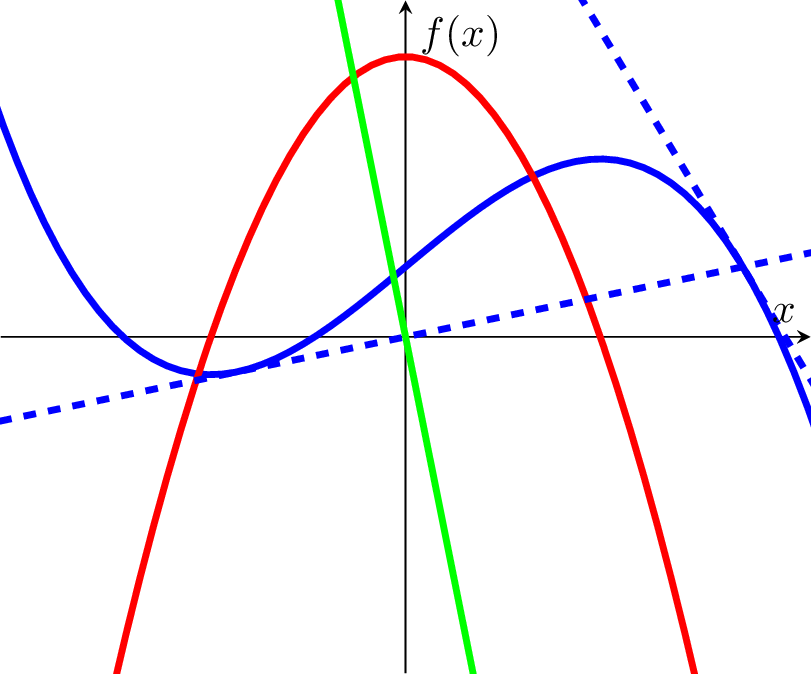
\includegraphics[width=1\linewidth]{fig6}
\caption{График параболы $f(x) = -x^3 + x + 0.25$ изображён синей кривой. Красной кривой обозначен график первой производной $f'(x) = -3x^2+1$, а зелённым цветом нарисована вторая производная $f''(x) = -6x$. Синей штриховкой нарисованы касательные к графику функции.}
\label{fig:71}
\end{figure}

\par Были использованы слова "выпукл" и "вогнут", может появиться вопрос, что они значат? Интуитивно понятно, что вогнутый на данном интервале график есть график, который как бы выталкивают на данном интервале в положительном направлении оси ординат, а выпуклый (иногда используется просторечие "впуклый") график~\----~выталкивают в направлении отрицательных значений оси ординат. Если же подходить к данному вопросу строго, то функция называется вогнутой на данном интервале, если для каждой точки данного интервала график находится ниже касательной, проведённой к точке данного интервала. А выпуклой на некотором интервале называется функция такая, что график находится выше касательной. Данные определения могут быть проиллюстрированы касательными на рисунке \ref{fig:71}. 

\subsection{Полином, факториал и дифференциальные уравнения}
Исследуем производные больших порядков от приведённого полинома степени $n$

\begin{equation}
	f(x) = x^n + a_{n-1} x^{n-1} + \ldots + a_1 x + a_0.
\end{equation}

Будет действовать последовательно. Сперва рассмотрим первую производную, тогда получим

\begin{equation}
	f'(x) = nx^{n-1} + a_{n-1} (n-1) x^{n-2} + \ldots + a_1.
\end{equation}

Степень полученного полинома меньше на единицу степени исходного полинома. Продолжаем вычислением второй производной, которая записывается следующим образом:

\begin{equation}
	f''(x) = f^{(2)}(x) = n (n-1) x^{n-1} + a_{n-1} (n-1) (n-2) x^{n-3} + \ldots + a_2.
\end{equation}

В данном выражении использованы обозначения Лагранжа для производных, которая заключается в том, что производная $m$\--ого порядка (то есть в выражении снизу $m$ штрихов) обозначается так:

\begin{equation}
	f{}' {}' {}^{\ldots}(x) = f^{(m)}(x).
\end{equation}

Итак, рассмотрим теперь $n$\--ую производную. Так как при взятии каждой последующей производной степень полинома всё больше и больше сокращается, то результатом взятия $n$\--ой производной будет константа. Так как при взятии каждой новой производной уходят члены, которые в исходном полиноме были членами степени, меньшей, чем номер берущийся производной, то при взятии $n$\--ой производной останется лишь первый член (он соответсвовал в исходном полиноме $x^n$). Данный член при каждом дифференцировании умножался на степень, а степень $x$ при этом уменьшалась на единицу. Таким образом, получаем следующий результат:

\begin{equation}
	f^{(n)}(x) = n(n-1)(n-2)\ldots2\cdot 1 = n!.
\end{equation}

Производные же более высоких порядков будут равняться тождественным нулям, так как

\begin{equation}
	f^{(n)}(x) \equiv \const,
\end{equation}

а производные от констант равны тождественно нулю. Данные соображения наводят на следующую теорему.

\begin{theorem}
	Если для функции $f(x)$ справедливо, что она дифференцируема $(n+1)$ раз и

	\begin{equation}
		f^{(n+1)}(x) \equiv 0,
	\end{equation}

	то $f(x)$ является многочленом степени не большей, чем $n$.
\end{theorem}

То есть полиномы степени $n$ являются решениями следующего так называемого дифференциального уравнения:

\begin{equation}
		f^{(n+1)}(x) \equiv 0.
\end{equation}

Под дифференциальным уравнением понимают выражение, содержащие суперпозицию производных функций, решением которого является некоторый набор функций. То есть, в отличие от алгебраических уравнений, тут решением является функциональная зависимость, а не число.

\section{Поиск нулей и особых точек}
Применим на практике знания, полученные выше. Рассмотрим многочлен третьей степени

\begin{equation}
	f(x) = x^3 + x^2 -x -1.
\end{equation}

Требуется найти нули, точки экстремума, точки перегиба и построить график данного многочлена.

\subsection{Поиск корней многочлена} % (fold)
Начнём с поиска корней многочлена. Рассматриваемый многочлен имеет третью степень, а, значит, существуют общая формула, называемая формулой Кардано \cite{root3}, для нахождения корней многочлена третьей степени. Однако данная формала крайне громоздка и не будет нами использована.

\par Рассматриваемый многочлен допускает нахождение как минимум одного корня способом угадывания. Действительно, если просто подставить $x=1$, то можно увидеть, что многочлен занулился. Значит, нами найден первый корень многочлена

\begin{equation}
 	x_1 = 1.
 \end{equation} 

Чтобы найти следующие корни, нужно поделить исходный многочлен третьей степени на линейный двучлен $x-x_1$, то есть на $x-1$. Деление столбиком продемонстрировано на рисунке \ref{fig:72}.

\begin{figure}[htbp]
	\centering
	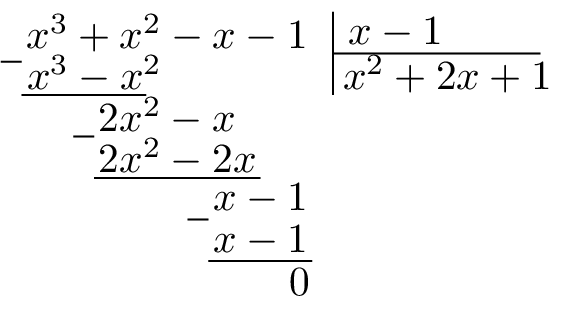
\includegraphics[width=\linewidth]{fig7}
	\caption{Деление столбиком многочлена $x^3+x^2-x-1$ на линейнай двучлен $x-1$.}
	\label{fig:72}
\end{figure}

Таким образом, мы приходим к тому, что осталось разрешить простое квадратное уравнение. Ведь исходный полином третьей степени поделился без остатка на $x-1$, что равноценно записи

\begin{equation}
	x^3+x^2-x-1 = (x-1)\cdot(x^2+2x+1).
\end{equation}

Отсюда и следует, что корни полинома

\begin{equation}
	x^2 + 2x +1
\end{equation}

будут корнями и исходного многочлена. Пользуемся формулами сокращенного умножения и записываем полученный квадратный трёхчлен в следующей форме:

\begin{equation}
	x^2 + 2x +1 = (x+1)^2.
\end{equation}

Отсюда сразу становится видно, что следующим корнем будет число $-1$, но это будет корень кратности два, что отражается в такой записи:

\begin{equation}
	x_2 = x_3 = -1.
\end{equation}
% subsection поиск_корней_многочлена (end)

\subsection{Поиск локальных экстремумов} % (fold)
Как было показано ранее, чтобы найти локальные экстремумы, нужно приравнять первую производную от функции к нулю. В нашем случаем имеем следующее уравнение на экстремумы:

\begin{equation}
	f'(x) = 3x^2 +2x - 1 = 0.
\end{equation}

Разрешить полученное квадратное уравнение не составляет труда. Получаем корни 

\begin{equation}
	x = -1;\ \dfrac{1}{3}. 
\end{equation}

Из предыдущих результатов ясно, что 

\begin{equation}
	f(-1) = 0,
\end{equation}

а значение в точки $1/3$ нужно вычислять, оно составляет

\begin{equation}
	f\qty(\dfrac{1}{3}) = -\dfrac{32}{27}.
\end{equation}
% subsection поиск_локальных_экстремумов (end)

\subsection{Точки перегиба} % (fold)
\label{sec:53}
Чтобы завершить исследование функции, осталось лишь исследовать её на выпуклость и вогнутость и найти в каких точках одно переходит в другое, если вообще переходит. Для этого потребуется вычислить вторую производную. Производя несложные вычисления, находим, что 

\begin{equation}
	f''(x) = 6x + 2.
\end{equation}

Таким образом, точкой перегиба будет точка $x = -1/3$, до неё (при $x< -1/3$) график функции вогнутый, а после~\----~выпуклый. Результат наших изысканий отображён на рисунке \ref{fig:73}.

\begin{figure}[htbp]
	\centering
	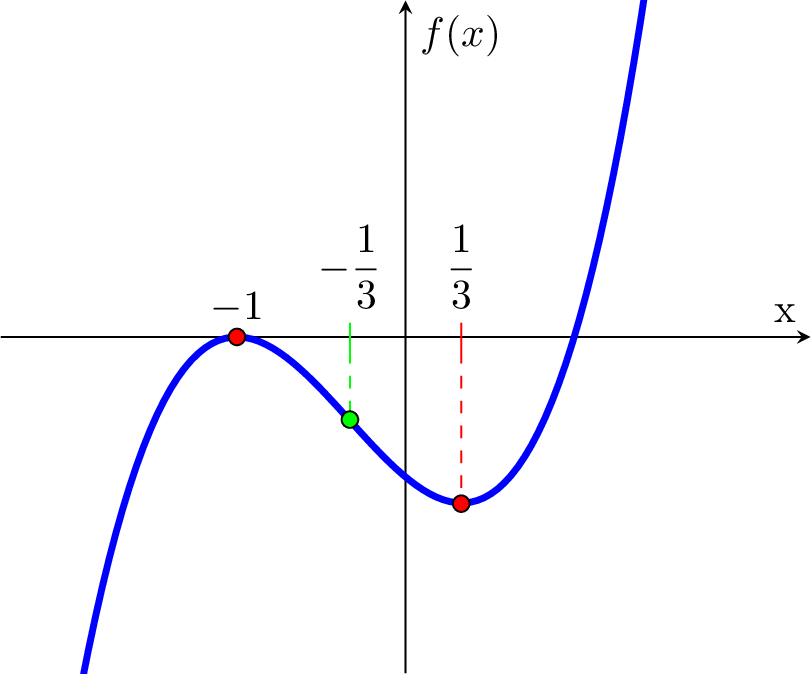
\includegraphics[width=\linewidth]{fig8}
	\caption{График функции $x^3 + x^2 - x -1$. Красными точками отображены экстремумы функции. Зеленой точке соответсвует точка перегиба.}
	\label{fig:73}
\end{figure}
% subsection точки_перегиба (end)

\section{Локальные максимумы и минимумы} % (fold)
\label{sec:6}
Исследуем на локальные максимумы и локальные минимумы функцию 

\begin{equation}
	f(x) = x^4(1-x)^2 = x^6-2x^5+x^4.
\end{equation}

Прежде всего найдём экстремумы из равенства нулю первой производной. Первая производная выглядит следующим образом:

\begin{equation}
	f'(x) = 6x^5 -10x^4+4x^3.
\end{equation}

Ясно, что одним из корней $f'(x)$ будет являться нуль, он будет иметь кратность, равную тройке, тогда остальные корни будут корнями квадратного трехчлена. Эти слова значат буквально следующее:

\begin{equation}
	f'(x) = 6x^5 -10x^4+4x^3 = 2x^3(3x^2 - 5x + 2).
\end{equation}

Отсюда сразу видно, что корнями полинома будут

\begin{equation}
	x_1 = x_2 = x_3 = 0,\quad x_4 = 1, \quad x_5 = \dfrac{2}{3},
\end{equation}

в чём читатель может убедиться самостоятельно. Эти точки являются подозрительными на точки локального максимума или локального минимума. Одним из способов разрешения данных подозрений является оценка знака второй производной в подозреваемых точках. Тогда вычисляем вторую производную и получаем результат

\begin{equation}
	f''(x) = 30 x^4 -40x^3+12x^2. 
\end{equation}

Если подставить в данное выражение $x=0$, то получим 

\begin{equation}
	f''(0) = 0,
\end{equation}

что означает, что мы до сих пор не можем ничего сказать о точке $x=0$, можем лишь констатировать, что требуется более глубокий анализ. Если же подставить точку $x=2/3$, то 

\begin{equation}
	f''\qty(\dfrac{2}{3}) = \qty(\dfrac{2}{3})^2(30 \cdot \dfrac{4}{9} - 40 \cdot \dfrac{2}{3} + 12) = \qty(\dfrac{2}{3})^2 \cdot \qty(-\dfrac{4}{3}) < 0.
\end{equation}

Видно, что вторая производная в данной точке имеет отрицательное значение, отсюда следует, что точка $x=2/3$ находится локальный максимум.

\par А для точки $x=1$ читатель может самостоятельно убедиться в том, что вторая производная в данной точке будет положительной, значит, в точке располагается локальный минимум.

\par Осталось разобраться с точкой $x=0$. Для этого рассмотрим старшие производные. Начнём с третьей производной

\begin{equation}
	f'''(x) = 120 x^3 - 120x^2 + 24x.
\end{equation}

Очевидно, что третья производная тоже зануляется в точке $x=0$. Если бы это было не так и третья производная не занулилась, то можно было бы сказать, что в окрестности точки $x=0$ функция устроена как $x^3$, то есть рост, например, в ней замедляется, а после прохода $x=0$ рост начинает ускоряться. Рассмотрим четвёртую производную

\begin{equation}
	f''''(x) = 360x^2-240x+24.
\end{equation}

Данная производная уже не зануляется. Она в точке нуль положительна и равна $24$. Это означает, что в окрестность $x=0$ функция устроена очень плоско, как $x^4$. То есть в точке $x=0$ находится локальный минимум. В результате исследования функции были найдены точки экстремума и можно построить её график (см. рис. \ref{fig:74}). Важно, заметить, что функция не ограничена сверху, поэтому у неё нет глобального максимума, в то время, как глобальному минимуму соответсвуют целых две точки~\----~точки лонального минимума. 

\begin{figure}[htbp]
	\centering
	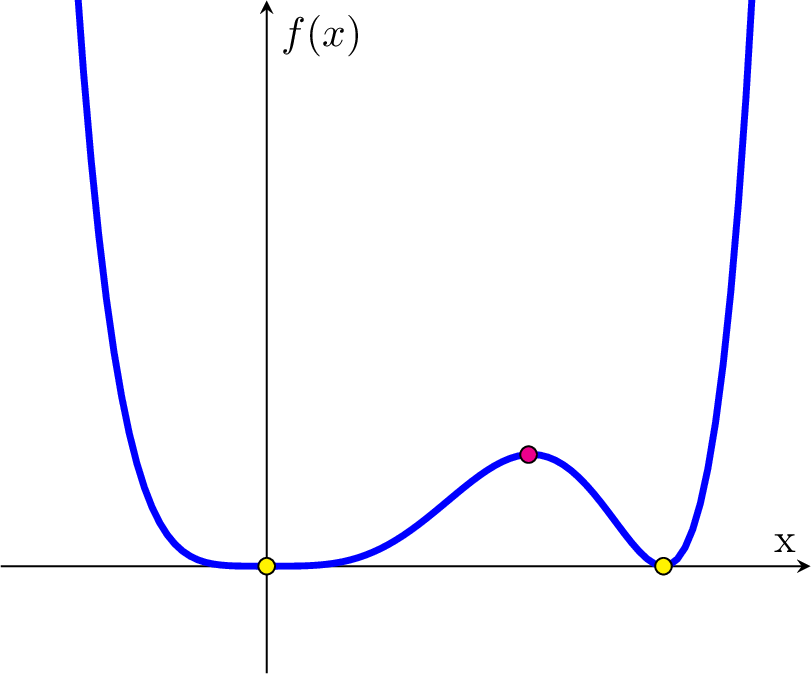
\includegraphics[width=\linewidth]{fig9}
	\caption{График функции $x^6-2x^5+x^4$. Желтыми точками отображены локальные минимумы функции, которые являются и глобальными минимума. Пурпурной точке соответсвует точка локального максимума.}
	\label{fig:74}
\end{figure}
% section локальные_ (end)

\section{Построение графика функции} % (fold)
Будем исследовать функцию отличную от многочлена, а именно

\begin{equation}
	f(x) = \dfrac{1}{x} - \dfrac{1}{x^2}.
\end{equation}

Ясно, что область определения данной функции представляет из себя

\begin{equation}
	\qty{\mathbb{R} - \qty{0}},
\end{equation}

то есть все действительные числа, кроме нуля, умеют отображаться данной функцией во множество действительных чисел.

\par Если привести функцию к общему знаменателю, то удастся найти её нуль

\begin{equation}
	f(x) = \dfrac{1}{x} - \dfrac{1}{x^2} = \dfrac{x - 1}{x^2}.
\end{equation}

Нулём функции будет тока $x_1 = 1$. Посчитаем производную

\begin{equation}
	f'(x) = \dfrac{1}{x^2} + \dfrac{2}{x^3} = \dfrac{2-x}{x^3}.
\end{equation}

Точкой, подозрительной на экстремум, будет точка $x=2$. Для того, чтобы определить является ли она точкой экстремума или нет, а если да, то каким, обратимся к оценке знака первой производной. При $x<0$ первая производная положительна, на интервале $ 0 < x \le 2$ она отрицательная и при $x>2$ снова положительна. Значит, точка $x=2$ является точкой локального максимума.

\par Исследуем асимптотику функции. Если $x$ стремится к минус бесконечности, то 

\begin{equation}
	f(x) = \dfrac{x - 1}{x^2} \underset{x\rightarrow-\infty}{\longrightarrow} -0.
\end{equation}

То есть из\--за того, что функция убывает по модулю при стремлении $x$ к минус бесконечности и остаются при этом отрицательной, она будет графически подходить снизу к оси абсцисс при уменьшении аргумента. Если же стремить $x$ к нулю слева, то

\begin{equation}
	f(x) = \dfrac{x - 1}{x^2} \underset{x\rightarrow-0}{\longrightarrow} -\infty.
\end{equation}

Аналогичные результаты получаются при исследовании асимптотики для положительных $x$:

\begin{gather} 
f(x) = \dfrac{x - 1}{x^2} \underset{x\rightarrow+0}{\longrightarrow} -\infty; \\ 
f(x) = \dfrac{x - 1}{x^2} \underset{x\rightarrow +\infty}{\longrightarrow} +0.
\end{gather}

Исследуем теперь нашу функцию на точки перегиба. Для этого приравняем к нулю вторую производную

\begin{equation}
	f''(x) = \dfrac{2}{x^3} - \dfrac{6}{x^4} = 0.
\end{equation}

Решением уравнения на точку перегиба является $x=3$. В данной точке вогнутость сменяется на выпуклость. Наши рассуждения совершенно справедливы, что можно подтвердить непосредственным построением графика (см. рис. \ref{fig:75}).


\begin{figure}[htbp]
	\centering
	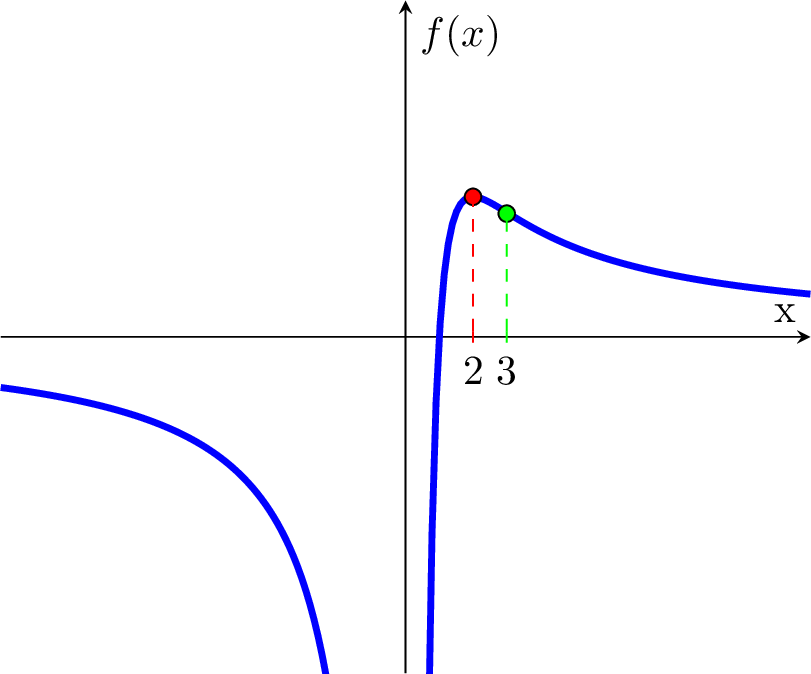
\includegraphics[width=\linewidth]{fig10}
	\caption{График функции ${1}/{x} - {1}/{x^2}$. Красной точкой обозначен максимум функции, зелёной~\----~точка перегиба.}
	\label{fig:75}
\end{figure}
% section построение_графика_функции (end)
\begin{thebibliography}{9}
	\bibitem{lim_use}
	Савватеев А., Тонис А., \textit{Применение пределов в математическом анализе}
	\\\texttt{\url{https://enabla.com/ru/pub/663}}
	
	\bibitem{poly_div}
	Wikipedia, \textit{Деление многочленов столбиком}
	\\\href{https://ru.wikipedia.org/wiki/\%D0\%94\%D0\%B5\%D0\%BB\%D0\%B5\%D0\%BD\%D0\%B8\%D0\%B5_\%D0\%BC\%D0\%BD\%D0\%BE\%D0\%B3\%D0\%BE\%D1\%87\%D0\%BB\%D0\%B5\%D0\%BD\%D0\%BE\%D0\%B2_\%D1\%81\%D1\%82\%D0\%BE\%D0\%BB\%D0\%B1\%D0\%B8\%D0\%BA\%D0\%BE\%D0\%BC}{https://ru.wikipedia.org/wiki/Деление\_многочленов\_столбиком}

	\bibitem{sok_um}
	Wikipedia, \textit{Формулы сокращенного умножения многочленов}
	\\\href{https://ru.wikipedia.org/wiki/\%D0\%A4\%D0\%BE\%D1\%80\%D0\%BC\%D1\%83\%D0\%BB\%D1\%8B\_\%D1\%81\%D0\%BE\%D0\%BA\%D1\%80\%D0\%B0\%D1\%89\%D1\%91\%D0\%BD\%D0\%BD\%D0\%BE\%D0\%B3\%D0\%BE\_\%D1\%83\%D0\%BC\%D0\%BD\%D0\%BE\%D0\%B6\%D0\%B5\%D0\%BD\%D0\%B8\%D1\%8F\_\%D0\%BC\%D0\%BD\%D0\%BE\%D0\%B3\%D0\%BE\%D1\%87\%D0\%BB\%D0\%B5\%D0\%BD\%D0\%BE\%D0\%B2}{https://ru.wikipedia.org/wiki/Формулы\_сокращенного\_умножения\_многочленов}

	\bibitem{root3}
	Wikipedia, \textit{Формула Кардано}
	\\\href{https://ru.wikipedia.org/wiki/\%D0\%A4\%D0\%BE\%D1\%80\%D0\%BC\%D1\%83\%D0\%BB\%D0\%B0\_\%D0\%9A\%D0\%B0\%D1\%80\%D0\%B4\%D0\%B0\%D0\%BD\%D0\%BE}{https://ru.wikipedia.org/wiki/Формула\_Кардано}
\end{thebibliography}
\end{document}
B4\%D0\%B0\%D0\%BD\%D0\%BE}{https://ru.wikipedia.org/wiki/Формула\_Кардано}
\end{thebibliography}
\end{document}
